\documentclass[11pt]{article}
\usepackage{geometry}\geometry{margin=1in}
\usepackage{amsmath, amssymb, amscd, amsthm, amsfonts}
\usepackage{todonotes, xspace}
\usepackage{enumitem}
\usepackage{tabularx}
\usepackage{multirow}

\usepackage{algorithm,algpseudocode}
% \usepackage{graphicx}
% \usepackage{hyperref}

\usepackage{xcolor}
\usepackage{listings}
% \usepackage{hyperref}
\usepackage[implicit=false]{hyperref}
\usepackage{courier}

\definecolor{mGreen}{rgb}{0,0.6,0}
\definecolor{mGray}{rgb}{0.5,0.5,0.5}
\definecolor{mPurple}{rgb}{0.58,0,0.82}
\definecolor{backgroundColour}{rgb}{0.95,0.95,0.92}

\lstdefinestyle{CStyle}{
    backgroundcolor=\color{backgroundColour},
    commentstyle=\color{mGreen},
    keywordstyle=\color{magenta},
    numberstyle=\tiny\color{mGray},
    stringstyle=\color{mPurple},
    basicstyle=\footnotesize,
    breakatwhitespace=false,
    breaklines=true,
    captionpos=b,
    keepspaces=true,
    numbers=left,
    numbersep=5pt,
    showspaces=false,
    showstringspaces=false,
    showtabs=false,
    tabsize=4,
    language=C
}


\newcommand{\EH}[2][inline]{\todo[color=orange!30,#1]{\sf \small\textbf{TODO:} #2\normalsize}\xspace}

\newcommand{\auton}{\textsc{FindTracklets}\xspace}


% \oddsidemargin 0pt
% \evensidemargin 0pt
% \marginparwidth 40pt
% \marginparsep 10pt
% \topmargin -20pt
% \headsep 10pt
% \textheight 8.7in
% \textwidth 6.65in
\linespread{1}

\title{An Evolutionary Algorithm for Near-Optimal Binary Search Tree Construction}

\author{Evan Hataishi\\ \small ICS 674: Evolutionary Computation\\ \small Prof. L. Altenberg}

\date{\small May 8, 2020}

\begin{document}

\maketitle

% \begin{abstract}
%
%     Given time series detections of moving objects in space, astronomers would like to identify asteroids and link those detections into a linear path within and between nights. Current algorithms use a series of 3-dimensional orthogonal range queries to link neighboring observations into such paths. A fast, efficient, and scalable data structure is needed to reduce the cost of these queries. In this work, we describe the currently used software which uses kd-trees. We then implement the theoretically faster range tree in an attempt to improve the overall performance. Using the same asteroid detection and linking software, we benchmark the kd-tree against our range tree implementation. We find that although just as accurate, the range tree performs much worse in practice for both tree construction time and query time compared to the kd-tree.
%
% \end{abstract}


\section{Introduction}
\label{sec-introduction}

Finding the optimal Binary Search Tree (BST) is a somewhat classical programming problem. Given a set of keys and a probability that each key will be looked up i.e. frequency, the optimal BST is structured s.t. the expected search time over all keys is minimized. The expected cost of searching for any arbitrary key is $frequency \times (depth + 1)$. The expected search time of the entire BST is simply the sum of the search costs of all keys. Specifically, the goal is to construct a BST that minimizes the expected search time, while maintaining BST properties given the key values. Thus, it is preferable to have keys with higher frequencies at a shorter depth. Figure~\ref{fig:opt-bst} shows 5 different BSTs that can be constructed given a set of keys (value row).

\begin{figure}[h]
    \centering
    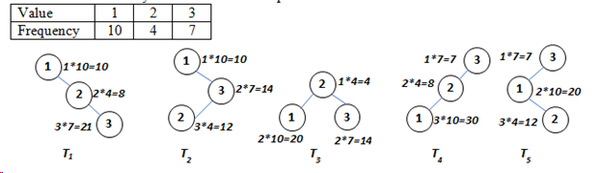
\includegraphics[width=0.9\columnwidth]{figures/opt_bst.png}
    \caption{ \small Various BST structures constructed from the same keys (reproduced from~\cite{bst_figure}).}
    \label{fig:opt-bst}
\end{figure}

A solution to the optimal BST problem is to simply try each key as root and recursively build each subtree. After exhaustively constructing every valid BST structure, the one with the minimum cost can be chosen. Given a tree with $n$ nodes, this would take exponential time to solve. However, this naive solution can be further improved to $O(n^3)$ with dynamic programming. Although finding the optimal BST structure for any arbitrary set of keys and frequencies has been bounded, we would like to explore the application of an evolutionary algorithm to this problem.

\subsection{Problem Statement}

Given a set of keys $k_1,k_2,\dots,k_n$ and a set of frequencies $f_1,f_2,\dots,f_n$ s.t. $f_i$ is the expected search frequency of $k_i$, we would like to use an evolutionary algorithm to construct a BST with minimal expected search time over all keys given the frequencies.



\section{Evolutionary Algorithm}
\label{sec-algorithm}

\begin{description}
    \item[Search Space] All valid BST structures.
    \item[Representation] An $N$ node BST constructed from a set of $N$ keys and a corresponding set of $N$ frequencies.
    \item[Objective Function] Let $k$ be the set of $N$ keys, and $f$ be the set of $N$ frequencies representing a BST. The expected cost of the BST can be calculated as follows:
    \begin{equation*}
        f(k, f) = \sum_{i=1}^{N} (depth(k_i) + 1) \times f_i.
    \end{equation*}
    Therefore, we aim to minimize the expected cost, which will be some non-zero value depending on keys and frequencies.
    \item[Variation Operators] Recombination is done by merging two trees and removing duplicate nodes. Recombination is only done using parents in the top 50\% of fitness. Mutation has a 10\% chance of occurring on any tree. The keys are simply shuffled and inserted to generate a new BST structure.
    \item[Selection Operator] We use elitism to pick the top 30\% of a generation to move on automatically to the next generation. The other 70\% is formed from recombination.
\end{description}

Keys are unique and randomly generated at the start. Frequencies are picked randomly between 1 and 10 (inclusive) for each key. Recombination is difficult, for merging trees can be tricky. While merging, the resulting tree must maintain the same set of keys with no duplicates. To do this, we take the set of keys for two trees (ordered by insertion order) and randomly take the index from one of the key pairs. We then ``flatten'' the list to obtain a new list of all the keys and no duplicates.



\section{Code}

To avoid having code within this report, all code used for this project can be found on my GitHub in a public repository~\cite{project_repository}. \texttt{BST.py} contains a class \texttt{BST}. All methods related to my genome representation are implemented within that class. \texttt{main.py} is a driver and runs the genetic algorithm. Within \texttt{main.py}, we first define some hyper-parameters: \texttt{TREE\_SIZE=100, POP\_SIZE=45, GENERATIONS=300, SELECT\_PERC=0.3}.

\subsection{Search Space Representation}

 \texttt{BST} has an attribute called \texttt{nodes}, which represents the order in which each node was inserted to construct the BST (used for recombination). The constructor: \texttt{\_\_init\_\_(self, data)} takes a list of pairs of keys and frequencies, creates a node for each pair, and inserts each node into the BST. Both keys and frequencies should take arbitrary values, so (unique) keys are simply generated from a range given the tree size, and a frequency for each key is a randomly generated integer between 0 and 10 inclusive. The set of keys is then re-shuffled (to create a random insertion order) to generate each new BST in the population.

 \subsection{Variation Operator Encoding}
Crossover is implemented as a static method: \texttt{crossover(p1, p2)}. Given two parents, it produces a single child by the crossover process described in Section~\ref{sec-algorithm}.

 \subsection{Selection Operator Encoding}
Selection is done in \texttt{main.py}. All agents are sorted by fitness, and the top 30\% are selected to move on to the next generation.

 \subsection{Termination Criterion}
We only terminate when either the optimal cost is reached. The actual optimal cost is calculated beforehand using a proven classical approach. However, the optimal is usually never found given the hyper-parameters, so we terminate at 300 generations.



\section{Results}

Figure~\ref{fig:results} shows the best, average, and worst genome fitness in the population over 500 generations. Since the optimal fitness value is a minimum, and larger fitness values mean a ``worse'' genome, we negate every fitness value to obtain a more intuitive graph with the minimum at the top. Results seem fairly typical for a genetic algorithm. Average and worst fitness values are messy and have a high variance across generations. The best fitness values converge fairly quickly and do not move around much. At the end of 500 generations, the best genome had a fitness of -1326. Using the classical algorithm given this set of keys and frequencies, the actual optimal value is -1224, so this seems fairly close.

\begin{figure}[h]
    \centering
    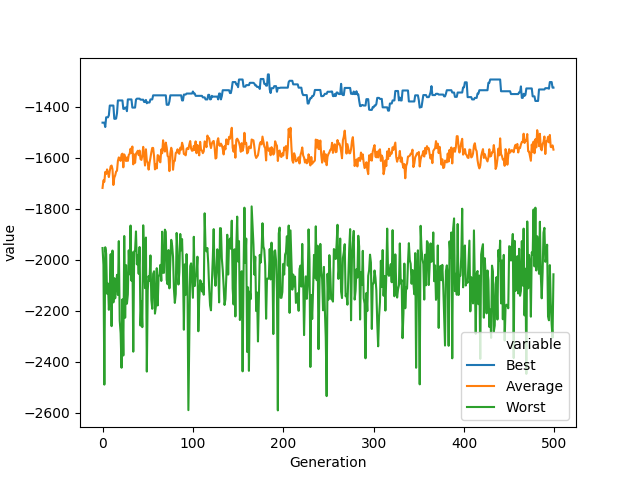
\includegraphics[scale=0.75]{figures/results.png}
    \caption{ \small Fitness results over 500 generations.}
    \label{fig:results}
\end{figure}


% 
\section{Conclusion}

We have proposed an evolutionary approach for constructing near-optimal binary search trees. Like some of the previous work discussed in Section~\ref{sec-relatedwork}, we use classical evolutionary techniques to setup the problem. The novelty of the algorithm proposed in this work is the way in which crossover is implemented. Rather than attempting to combine two BSTs based directly on their structures, we consider reducing each BST to a list of keys sorted by insertion order then doing crossover. We find that the algorithm converges fairly quickly (within a few hundred generations) and is able to construct a near-optimal BST.

\subsection{Future Work}
We can propose two main directions for future work. The first is to tune the algorithm parameters in the hopes of seeing slightly better convergence. A more major direction is to reconsider the way in which crossover is implemented.



\bibliographystyle{plain}
\bibliography{biblio}

\end{document}
